\documentclass[12pt,letter]{article}
\usepackage[moduleName={Mega Tone}]{KautenjaDSP}
% import a debugging package to show the margin boxes
% \usepackage{showframe}
% set the graphics path to the img directory
\graphicspath{{img/}}

% algorithm2e stuff
% \SetKwInOut{Objects}{$\CKmatrix{O}$}
% \SetKwInOut{Weights}{$\CKvector{w}$}

\begin{document}
\titlePage{MegaTone-Logo}{MegaTone-Module}{KautenjaDSP}

% -------------------
% MARK: Overview
% -------------------

\section{Overview}

Mega Tone is an emulation of the Texas Instruments SN76489 audio processing unit from the Sega Master System, Sega Mega Drive, and Sega Genesis. The SN76489 chip contains three pulse waveform generators and an LFSR-based noise generator that selects between pitched white-noise and static periodic noise. Mega Tone provides the key features of the SN76489 chip, namely,
\begin{itemize}
  \item \textbf{Triple Pulse Waveform Generator:} Three 8-bit pulse waves with $50\%$ duty cycle and 10-bit frequency parameter
  \item \textbf{Noise Generator:} Generate either pitched white-noise based on the frequency of oscillator three, or static periodic noise at one of three shift frequencies: $\frac{N}{2048}$, $\frac{N}{1024}$, $\frac{N}{512}$ where $N$ is the reference clock rate (which is something like $3579545Hz$).
  \item \textbf{4-bit Amplifier:} A 4-bit amplifier controls the output level of each oscillator with mixer sliders and CV inputs
\end{itemize}

% -------------------
% MARK: Panel Layout
% -------------------

\clearpage
\section{Panel Layout}

\begin{figure}[!htp]
\centering
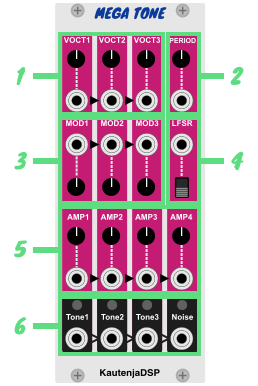
\includegraphics{MegaTone-Manual}
\end{figure}

\begin{enumerate}
  \item Coarse frequency control over the four oscillators. Frequency is quantized to a 10-bit value for the tone generators.
  \item $V$/Octave inputs for pulse waveform generators.
  \item linear CV frequency modulation for pulse waveform generators.
  \item LFSR switch. When pointing up, periodic noise is generated. When pointing down, pitched white noise is generated.
  \item CV LFSR gate, high at $2V$. Holds the LFSR generator as long as the input voltage is $>2V$. Inverts when LFSR switch is high.
  \item Noise generator shift rate. Select between one of four shift rates: the output of tone generator 3, $N / 512$, $N / 1024$, or $N / 2048$.
  \item Volume. Coarse amplitude control over the oscillators using the 4-bit amplifier. When no input is connected, the slider controls the level from $0\%$ to $100\%$. When an input is connected, the slider acts as an attenuator.
  \item Channel outputs, ${\approx}10V_{pp}$.
\end{enumerate}

% -------------------
% MARK: References
% -------------------

\clearpage
\renewcommand\refname{References \& Acknowledgments}
\nocite{*}
\bibliographystyle{apalike}
\bibliography{references}

\end{document}
